% This example is meant to be compiled with lualatex or xelatex
% The theme itself also supports pdflatex
\PassOptionsToPackage{unicode}{hyperref}
\documentclass[aspectratio=1610, 9pt]{beamer}

% Warning, if another latex run is needed
% \usepackage[aux]{rerunfilecheck}

% just list chapters and sections in the toc, not subsections or smaller
\setcounter{tocdepth}{1}

%------------------------------------------------------------------------------
%------------------------------ Fonts, Unicode, Language ----------------------
%------------------------------------------------------------------------------
\usepackage{fontspec}
\defaultfontfeatures{Ligatures=TeX}  % -- becomes en-dash etc.

% german language
\usepackage{polyglossia}
\setdefaultlanguage{german}

% for english abstract and english titles in the toc
\setotherlanguages{english}

% intelligent quotation marks, language and nesting sensitive
\usepackage[autostyle]{csquotes}

% microtypographical features, makes the text look nicer on the small scale
\usepackage{microtype}

%------------------------------------------------------------------------------
%------------------------ Math Packages and settings --------------------------
%------------------------------------------------------------------------------

\usepackage{amsmath}
\usepackage{amssymb}
\usepackage{mathtools}
\usepackage{bbold}

% Enable Unicode-Math and follow the ISO-Standards for typesetting math
\usepackage[
  math-style=ISO,
  bold-style=ISO,
  sans-style=italic,
  nabla=upright,
  partial=upright,
]{unicode-math}
\setmathfont{Latin Modern Math}

% nice, small fracs for the text with \sfrac{}{}
\usepackage{xfrac}


%------------------------------------------------------------------------------
%---------------------------- Numbers and Units -------------------------------
%------------------------------------------------------------------------------

\usepackage[
  locale=DE,
  separate-uncertainty=true,
  per-mode=symbol-or-fraction,
]{siunitx}
\sisetup{math-micro=\text{µ},text-micro=µ}
% \sisetup{tophrase={{ to }}}
%------------------------------------------------------------------------------
%-------------------------------- tables  -------------------------------------
%------------------------------------------------------------------------------

\usepackage{booktabs}       % \toprule, \midrule, \bottomrule, etc

%------------------------------------------------------------------------------
%-------------------------------- graphics -------------------------------------
%------------------------------------------------------------------------------

\usepackage{graphicx}
%\usepackage{rotating}
\usepackage{grffile}
\usepackage{tikz}
\usepackage{circuitikz}
\usepackage{tikz-feynman}
\usepackage{subcaption}

% allow figures to be placed in the running text by default:
\usepackage{scrhack}
\usepackage{float}
\floatplacement{figure}{htbp}
\floatplacement{table}{htbp}

% keep figures and tables in the section
\usepackage[section, below]{placeins}


%------------------------------------------------------------------------------
%---------------------- customize list environments ---------------------------
%------------------------------------------------------------------------------

\usepackage{enumitem}
\usepackage{listings}
\usepackage{hepunits}

\usepackage{pdfpages}
%------------------------------------------------------------------------------
%------------------------------ Bibliographie ---------------------------------
%------------------------------------------------------------------------------

\usepackage[
  backend=biber,   % use modern biber backend
  autolang=hyphen, % load hyphenation rules for if language of bibentry is not
                   % german, has to be loaded with \setotherlanguages
                   % in the references.bib use langid={en} for english sources
]{biblatex}
\addbibresource{references.bib}  % the bib file to use
\DefineBibliographyStrings{german}{andothers = {{et\,al\adddot}}}  % replace u.a. with et al.


% Load packages you need here
% \usepackage{polyglossia}
% \setmainlanguage{german}

\usepackage{csquotes}


% \usepackage{amsmath}
% \usepackage{amssymb}
% \usepackage{mathtools}

\usepackage{hyperref}
\usepackage{bookmark}

% load the theme after all packages

\usetheme[
  showtotalframes, % show total number of frames in the footline
]{tudo}

% Put settings here, like
\unimathsetup{
  math-style=ISO,
  bold-style=ISO,
  nabla=upright,
  partial=upright,
  mathrm=sym,
}

%Titel:
\title{The Muon Puzzle}
%Autor
\author[N.Breer]{Nils Breer}
%Lehrstuhl/Fakultät
\institute{Fakultät Physik}
%Titelgrafik muss ich einfueren!!!
%\titlegraphic{\includegraphics[width=0.3\textwidth]{content/Bilder/interferenz.jpg}}
\date{17.06.2022}

\begin{document}
\maketitle

\begin{frame}\frametitle{Agenda}
  \begin{itemize}
    \item What is the Muon Puzzle?
    \item Why do we want to study it?
    \item Cosmic rays and their behaviour with the atmosphere
    \item air shower: trivia and properties
    \item How do we measure these phenomena and which experiments are used?
    \item Other problems related to the muon puzzle
    \item possible solutions
  \end{itemize}
\end{frame}

\begin{frame}\frametitle{The Muon Puzzle}
  \begin{itemize}
    \item indirect observation of cosmic rays through air showers in atmosphere
    \item interpretation -> accurate models of air shower physics (QCD extreme)
    \item air showers -> hadronic cascades rich in muons
    \item $N_\mu$ key observable for mass composition of CR
    \item Simulation shows drastic Muon deficit compared to measurement! -> why?
    \item visible at TeV scale -> LHC also didn't observe that!
  \end{itemize}
\end{frame}

\begin{frame}\frametitle{Why is solving the puzzle interesting}
  \begin{itemize}
    \item reduce the size of $N_\mu$ bands by a factor of 2.5 to 4
    \item resolve ambiguity (mehrdeutigkeit) of cosmic ray mass composition at EeV level
    \item improve hadronic interaction models for CR mass composition in simulation
    \item more precision of lepton flux, main background for IceCube
  \end{itemize}
\end{frame}

\begin{frame}{flux}
  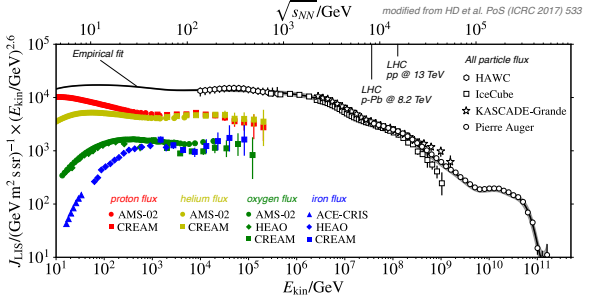
\includegraphics[width=\textwidth]{knee_heel.png}
\end{frame}

\begin{frame}{heel and knee plot, flux}
  \begin{itemize}
    \item Flux is scaled with $E^{2.6}$ -> many orders of magnitude
    \item open sybols: shower experiments measurring "all particle CR flux"
    \item coloured: flux of individual balloon and satelite measurements
    \item empirical fit to the data (what is empirical?)
    \item interesting part from above the knee at $\SI{1e6}{\giga\electronvolt}$.
  \end{itemize}
\end{frame}

\begin{frame}\frametitle{What are cosmic rays?}
  \begin{itemize}
    \item discovered by Victor Hess in 1912 (balloon experiment)
    \item Fully ionised nuclei, from protons up to iron, negligible fractions
    to higher nuclei
    \item arriving earth with relativistic energies
    \item come from unknown sources outside the solar system
    \item shock acceleration (< 1 PeV) in SNR, higher energies have unknown
    mechanisms, extra-galactic > 1 EeV
    \item "Knee" spectrum CR occur 1 per $m^2$ per year
    \item "Ankle" spectrum CR occur 1 per $\text{km}^2$ per century -> hard to study
  \end{itemize}
\end{frame}

\begin{frame}\frametitle{More about cosmic rays}
  \begin{itemize}
    \item CR may come from point-like sources, don't appear as such -> isotropic flux
    \item charged and scattered through inhomogenous fields -> random arrival directions
    \item E < 100 TeV: directly observed by space-based experiments (AMS-02\footnote{Alpha Magnetic Spectrometer})
    \item higher energies: flux too low -> ground based experiments
    (Auger, Telescope Array) through particle showers
  \end{itemize}
\end{frame}

\begin{frame}{Pierre Auger Observatory}
  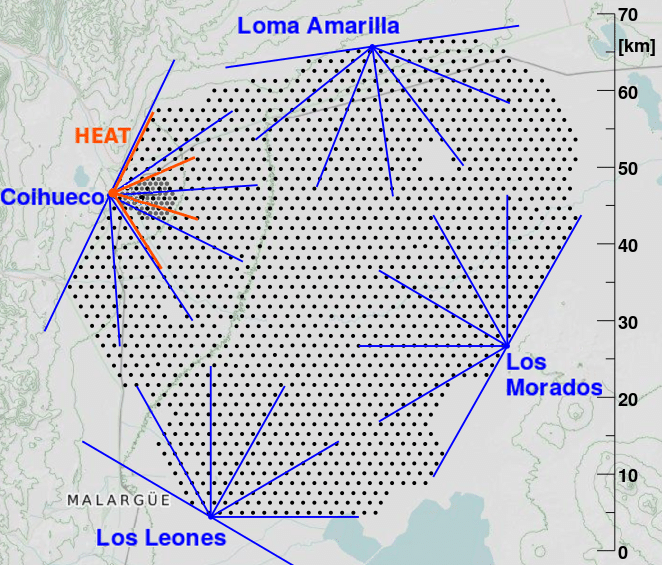
\includegraphics[width=\textwidth]{pierre.png}
\end{frame}

\begin{frame}\frametitle{Pierre Auger Experiment}
  \begin{itemize}
    \item located in Argentina
    \item CR Energies between $\num{1e17}$ and $\num{1e20}$ eV
    \item studies particle interactions with water tanks at surface
    \item tracking air showers through UV light in atmosphere
  \end{itemize}
\end{frame}

\begin{frame}{The Telescope Array}
  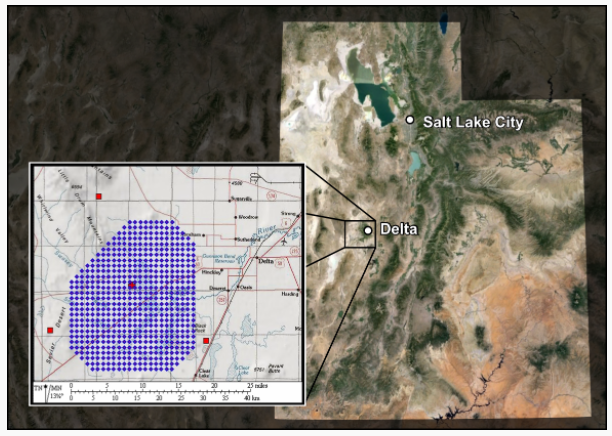
\includegraphics[width=\textwidth]{TCA.png}
\end{frame}

\begin{frame}\frametitle{Telescope Array}
  \begin{itemize}
    \item hybrid experiment from many collaborations
    \item observe air showers from CR at highest energies
    \item combination of air-flourescence (atmospheric trace) and groundbased
    \item scintillating trackers (footprint when reaching the surface)
  \end{itemize}
\end{frame}

\begin{frame}\frametitle{Air Showers}
  \begin{itemize}
    \item picture?
    \item description
    \item more details
  \end{itemize}
\end{frame}

\begin{frame}\frametitle{logarithmic mass prediction}
  \begin{columns}
    \begin{column}[c]{0.48\textwidth}
      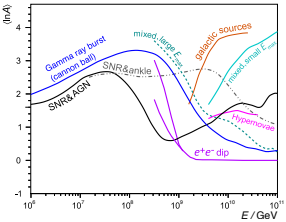
\includegraphics{lnA_left.png}
    \end{column}
    \begin{column}[c]{0.48\textwidth}
      \begin{itemize}
        \item search dominant sources of CR -> for low fluxes need air showers
        \item Air showers are indirectly observed and mass composition can only be sumarized by the logarithmic mass ln(A) (for E above PeV)
        \item -> why? because of the intrinsic fluctuations inside the air showers
        \item ln(A) for several source classes shown
        \item precise measurements can rule out competing theories (e.g CR with highest energies are light or heavy)
      \end{itemize}
    \end{column}
  \end{columns}
\end{frame}

\begin{frame}\frametitle{logarithmic mass prediction}
  \begin{columns}
    \begin{column}[c]{0.48\textwidth}
      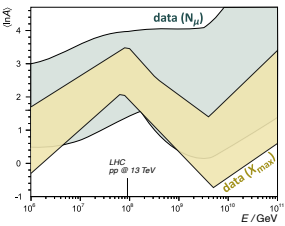
\includegraphics{lnA_right.png}
    \end{column}
    \begin{column}[c]{0.48\textwidth}
      \begin{itemize}
        \item bands constructed from several measurements on air showers
        \item mass-sensitive features: shower depth maximum $X_{max}$ and muon Number $N_{\mu}$
        \item band width \to theoretical uncertainties (forward hadron production)
        \item uncertainties prevent exclusion of theories on the CR origin
        \item $N_{\mu}$ good discrimination between light and heavy rays at EeV scale
        \item more usefull than $X_{max}$ because of few statistics of flourescence
        \item experimental uncertainy is 10\percent
      \end{itemize}
    \end{column}
  \end{columns}
\end{frame}

\begin{frame}\frametitle{experimental uncertainty measurements}
  \begin{columns}
    \begin{column}[c]{0.48\textwidth}
      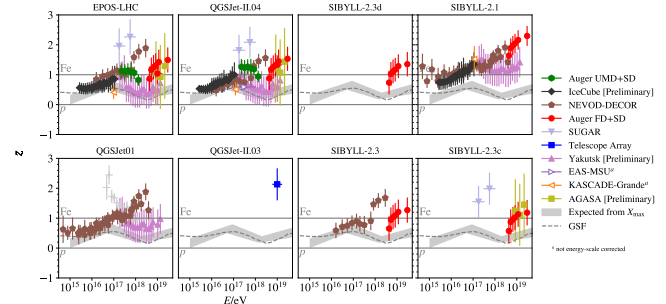
\includegraphics{unc.png}
    \end{column}
    \begin{column}[c]{0.48\textwidth}
      \begin{itemize}
        \item precise air shower measurements
        \item experimental uncertainty is 10\percent
        \item factor 2.5 to 4 (E dependent) small than band width (theoretical unc.)
        \item theo. unc. comes from shower simulation used to infer $ln(A)$ from $X_{max}$ and $N_{\mu}$
        \item simulation essential: no way of calibrating since mass composition of any astrophysical source unknown
        \item uncertainty from evolution of hadronic cascades; responsible for muon production at the end!
      \end{itemize}
    \end{column}
  \end{columns}
\end{frame

\begin{frame}{Now what is puzzling?}
  \begin{itemize}
    \item LHC has state-of-the-art softhadronic interaction models $=$ generators
    \item generators always predict a lower muon Number than seen in measurements
    \item prediction is nearly model-independent \to only small wiggle room
    \item Muon discrepancy starts right after the "knee", increases with $ln(shower E)$
    \item Discrepancy also seen in showers where first interaction of the CR has cms $=$ 8 TeV
    \item why not observed yet al LHC?
    \item have not looked at the right spot! wrong eta range for soft hadronic interactions (eta >= 2)
  \end{itemize}
\end{frame}

\begin{frame}\frametitle{Muon Messungen und Modelle}
  \begin{itemize}
    \item d
  \end{itemize}
\end{frame}

\begin{frame}{more to $N_\mu$}
  \begin{itemize}
    \item $N_\mu$ is sensitive to energy fraction of carried away photons from $\pi_0$ decays
    \item ALICE saw universal strangeness enhancement in final states, resulting in less pions in mid rapidity range
    \item this was only seen in heavy ion collisions! hint?
  \end{itemize}
\end{frame}

%%% hier muss siunitx eingebunden werden
\begin{frame}\frametitle{Possible solutions to the Puzzle}
  \begin{itemize}
    \item use LHCb as instrumentation device because it has the correct eta range (2 to 5)
  \end{itemize}
\end{frame}

\begin{frame}\frametitle{Recap}
  \begin{itemize}
    \item Muon deficit clearly visible in air showers with 8\sigma
    \item IceCube and the Pierre Auger experiment made huge contributions to model-dependent measurements
    \item $\sqrt{S_{NN}} \approx \SI{8}{\tera\electronvolt}$with linear increase in $\symup{log}(E)$ -> high energy measurements at LHC
    \item small modifications in hadron production reduce energy contribution of photons, coming from $\pi^{0}$ decays
  \end{itemize}
\end{frame}

\begin{frame}\frametitle{Quellen}
\url{http://www.telescopearray.org/index.php/about/telescope-array} \\
\url{https://www.researchgate.net/figure/A-schematic-of-the-Pierre-Auger-Observatory-where-each-black-dot-is-a-water-Cherenkov_fig1_319524774} \\
% \url{http://antares.in2p3.fr/} \\
% \url{https://ecap.nat.fau.de/index.php/research/neutrino-astronomy/antares-km3net/} \\
% \url{http://www.km3net.org/} \\
% \url{https://baikalgvd.jinr.ru/} \\
% \url{https://masterok.livejournal.com/2364208.html} \\
% \url{https://arxiv.org/pdf/1412.5106.pdf} \\
% \url{https://www.epj-conferences.org/articles/epjconf/pdf/2019/14/epjconf_ricap2019_01015.pdf} \\
% \url{https://pos.sissa.it/358/890/pdf} \\
\end{frame}

\end{document}

% \begin{frame}\frametitle{}
%   \begin{columns}
%   \begin{column}[c]{0.45\textwidth}
%     \begin{itemize}
%       \item
%       \item
%       \item
%       \item
%     \end{itemize}
%   \end{column}
%   \begin{column}[c]{0.45\textwidth}
%     % \includegraphics{images/icecube.png}
%   \end{column}
%   \end{columns}
% \end{frame}
